% Experiments: text quality across 33 languages, with baselines and ablation. Owner: claude (mnist/site thread, 2026-11-04). Additive to text_quality.tex.
\subsection{Text quality across 33 languages, against single-statistic baselines}
\label{sec:text-33}

Section~\ref{sec:text-quality} evaluated eight languages. Here the same protocol (first
300 kept and 300 removed documents of the first FineWeb-2 shard, AUC for kept $>$
removed) is run on 33 languages across eleven scripts (\texttt{examples/text\_quality/eval\_fineweb2.py};
Persian is not published in this layout and was skipped). As baselines, the same
documents are scored with single statistics of the kind used by rule-based filters
\cite{rae2021gopher,raffel2020t5}: $\log$ length, the fraction of characters that are
letters, the fraction of tokens containing a letter, and the Gopher-style distance of the
mean word length from 5.

\begin{figure}[t]\centering
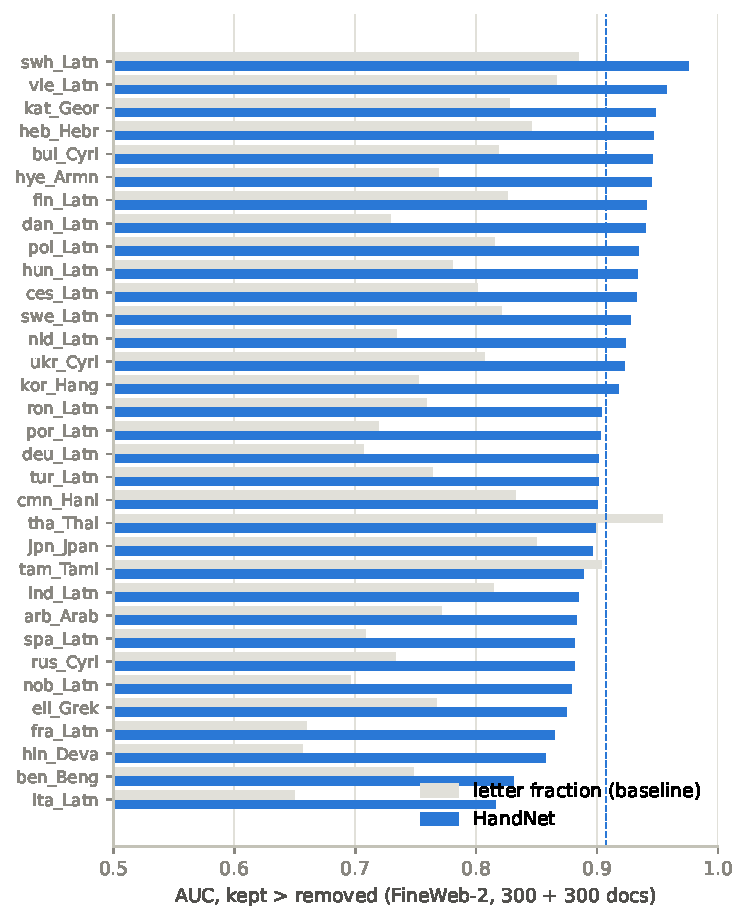
\includegraphics[width=0.62\linewidth]{figures/fineweb2_auc}
\caption{AUC(kept $>$ removed) per language, the text-quality network versus the
letter-fraction baseline. Dashed line: mean over languages (0.907).}
\label{fig:auc}
\end{figure}

\begin{table}[t]\centering\footnotesize
\caption{FineWeb-2 kept vs removed, 300 + 300 documents per language. AUC for the
text-quality network and for three single-statistic baselines; mean network score of
kept and removed documents.}
\label{tab:fineweb}
\begin{tabular}{lrrrrrr}
\toprule
language & network & length & letters & words & kept mean & removed mean \\
\midrule
swh\_Latn & 0.976 & 0.736 & 0.885 & 0.902 & 92.2 & 44.8 \\
vie\_Latn & 0.958 & 0.698 & 0.866 & 0.915 & 92.9 & 63.7 \\
kat\_Geor & 0.949 & 0.697 & 0.827 & 0.858 & 95.2 & 58.4 \\
heb\_Hebr & 0.947 & 0.643 & 0.846 & 0.886 & 93.0 & 58.6 \\
bul\_Cyrl & 0.946 & 0.668 & 0.819 & 0.873 & 96.0 & 66.9 \\
hye\_Armn & 0.945 & 0.534 & 0.769 & 0.763 & 93.5 & 57.0 \\
fin\_Latn & 0.941 & 0.696 & 0.826 & 0.861 & 97.4 & 64.8 \\
dan\_Latn & 0.940 & 0.657 & 0.729 & 0.803 & 95.3 & 66.5 \\
pol\_Latn & 0.934 & 0.643 & 0.815 & 0.818 & 95.4 & 64.5 \\
hun\_Latn & 0.933 & 0.705 & 0.780 & 0.854 & 96.3 & 64.4 \\
ces\_Latn & 0.932 & 0.675 & 0.801 & 0.852 & 95.1 & 62.3 \\
swe\_Latn & 0.928 & 0.671 & 0.821 & 0.882 & 95.2 & 68.8 \\
nld\_Latn & 0.924 & 0.638 & 0.734 & 0.846 & 94.8 & 68.8 \\
ukr\_Cyrl & 0.923 & 0.668 & 0.807 & 0.853 & 95.7 & 64.7 \\
kor\_Hang & 0.918 & 0.492 & 0.752 & 0.850 & 80.4 & 41.5 \\
ron\_Latn & 0.904 & 0.631 & 0.759 & 0.836 & 93.6 & 68.7 \\
por\_Latn & 0.903 & 0.637 & 0.720 & 0.770 & 94.0 & 67.0 \\
deu\_Latn & 0.901 & 0.628 & 0.707 & 0.849 & 95.6 & 74.1 \\
tur\_Latn & 0.901 & 0.604 & 0.764 & 0.780 & 94.5 & 70.5 \\
cmn\_Hani & 0.900 & 0.559 & 0.832 & 0.709 & 91.1 & 62.2 \\
tha\_Thai & 0.899 & 0.571 & 0.955 & 0.862 & 85.6 & 64.3 \\
jpn\_Jpan & 0.896 & 0.533 & 0.850 & 0.749 & 90.8 & 61.3 \\
tam\_Taml & 0.889 & 0.682 & 0.904 & 0.881 & 96.0 & 73.6 \\
ind\_Latn & 0.885 & 0.631 & 0.815 & 0.796 & 95.3 & 75.3 \\
arb\_Arab & 0.883 & 0.612 & 0.771 & 0.832 & 88.6 & 64.4 \\
spa\_Latn & 0.882 & 0.651 & 0.708 & 0.787 & 94.2 & 74.3 \\
rus\_Cyrl & 0.881 & 0.607 & 0.733 & 0.805 & 95.9 & 75.8 \\
nob\_Latn & 0.879 & 0.593 & 0.696 & 0.783 & 94.8 & 71.7 \\
ell\_Grek & 0.875 & 0.646 & 0.767 & 0.854 & 94.1 & 69.6 \\
fra\_Latn & 0.865 & 0.659 & 0.659 & 0.805 & 94.1 & 74.2 \\
hin\_Deva & 0.857 & 0.604 & 0.656 & 0.733 & 91.9 & 71.3 \\
ben\_Beng & 0.831 & 0.599 & 0.748 & 0.775 & 93.8 & 74.6 \\
ita\_Latn & 0.816 & 0.650 & 0.650 & 0.722 & 93.1 & 76.4 \\
\midrule
\textbf{mean (33)} & \textbf{0.907} & 0.634 & 0.781 & 0.823 & & \\
\bottomrule
\end{tabular}
\end{table}

\begin{figure}[t]\centering
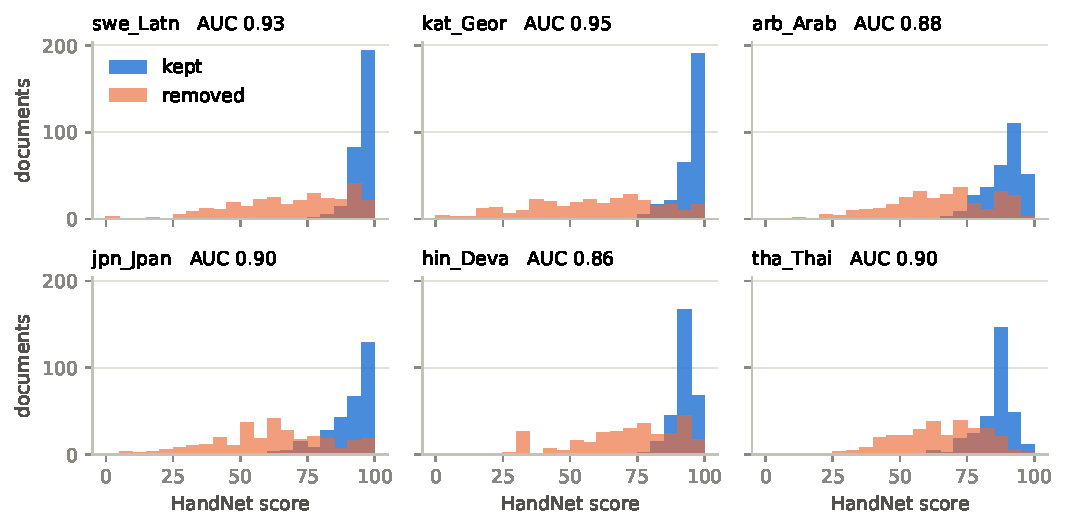
\includegraphics[width=\linewidth]{figures/fineweb2_hist}
\caption{Score distributions of kept (blue) and removed (orange) documents for six scripts.}
\label{fig:hist}
\end{figure}

Figure~\ref{fig:auc} and Table~\ref{tab:fineweb} give the results. The mean AUC is 0.907,
with every language above 0.81; Swahili (0.976), Vietnamese (0.958), Georgian (0.949),
Hebrew (0.947), Bulgarian (0.946) and Armenian (0.945) are highest, Italian (0.816),
Bengali (0.831) and Hindi (0.857) lowest. Scores of kept documents are tightly
concentrated near 95 while removed documents spread over the whole range
(Figure~\ref{fig:hist}); with a threshold of 50 essentially no kept document is rejected
in any language, and between 5\,\% (Italian) and 59\,\% (Korean) of removed documents
are.

Two observations. First, the letter fraction alone is a strong baseline (mean 0.78),
and for Thai it beats the network (0.955 vs 0.899): Thai has no sentence punctuation and
no word spaces, so the script gates switch off most of the structure detectors and little
is left. Second, FineWeb-2's own removal decisions are rule-based, so part of what is
measured is agreement between two rule systems rather than ground-truth quality; the
comparison still tells us that a 627-weight network reproduces most of a production
filtering pipeline's decisions in 33 languages.

In every language the most frequent penalties on removed documents are
\texttt{broken\_lines} (line breaks mid-sentence), \texttt{bullet\_lines} and
\texttt{fragments}, i.e.\ navigation lists and layout text, followed by
\texttt{few\_sentence\_ends} and \texttt{markup}.

\paragraph{Ablation over 33 languages.} Table~\ref{tab:ablation33} repeats the
leave-one-group-out ablation of Section~\ref{sec:text-quality} on all 33 languages, now
including the mixed-script penalty and the rewards
(\texttt{examples/text\_quality/ablate\_groups.py}). Only the \emph{formatting} group
matters much: without it the mean AUC drops from 0.907 to 0.858 and Thai from 0.90 to
0.69. The other groups are nearly redundant on this benchmark, and removing the
\emph{rewards} or the \emph{tokens} group slightly \emph{improves} the AUC. This is a
useful negative result for the design method: several detectors that are easy to
justify (shouting, digit runs, giant tokens) contribute nothing measurable to agreement
with FineWeb-2, and the reward units, which were meant to make the scale interpretable,
cost a little discrimination.

\begin{table}[t]\centering\small
\caption{Ablation over 33 languages: mean AUC with one group switched off.}
\label{tab:ablation33}
\begin{tabular}{lrrl}
\toprule
variant & mean AUC & $\Delta$ & worst language \\
\midrule
full & 0.907 & -- & 0.816 (ita\_Latn) \\
without noise & 0.905 & -0.003 & 0.810 (ita\_Latn) \\
without repetition & 0.904 & -0.003 & 0.809 (ita\_Latn) \\
without composition & 0.906 & -0.001 & 0.816 (ita\_Latn) \\
without formatting & 0.858 & -0.049 & 0.688 (tha\_Thai) \\
without tokens & 0.909 & +0.001 & 0.815 (ita\_Latn) \\
without structure & 0.906 & -0.002 & 0.820 (ita\_Latn) \\
without length & 0.905 & -0.003 & 0.806 (ita\_Latn) \\
without mixed\_scripts & 0.907 & -0.001 & 0.817 (ita\_Latn) \\
without reward & 0.913 & +0.006 & 0.830 (ita\_Latn) \\
\bottomrule
\end{tabular}
\end{table}
